\section{Dataset}
\label{sec:dataset}
The dataset consists of books from the 16\textsuperscript{th} and
17\textsuperscript{th} century. There are several peculiarities. Table
\ref{tab:statistics} shows that the amount of pages per book, and the amount of
images per book differs enormously per book.

Some examples of the pages can be seen in figure \ref{fig:textImageExamples},
\ref{fig:textExamples}, \ref{fig:imageExamples}, \ref{fig:qualityExamples} and
\ref{fig:baggerExamples}. Figure \ref{fig:qualityExamples} shows that there is
quite a large gap between the quality of scans of some books. The right image of
figure \ref{fig:qualityExamples}
has a vertical line, which indicates that both pages were scanned into the same
image. Furthermore, figure \ref{fig:baggerExamples} shows that some pages
contain something that we can not classify as text nor as an image.

\todo{spread this images out throughout the report. For example, we only need
one figure with text and image, which can be in the intro, and we can still
reference it from here}

\begin{figure}
\centering
    \begin{subfigure}[b]{0.4\textwidth}
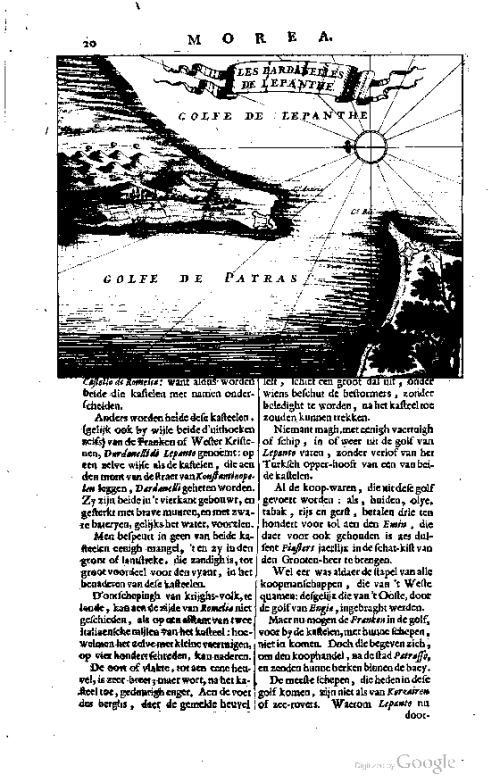
\includegraphics[width=\textwidth]{resources/pageImageExample}
    \end{subfigure}
    \begin{subfigure}[b]{0.4\textwidth}

\includegraphics[width=\textwidth]{resources/pageImageExample2}
    \end{subfigure}
    \caption{Examples of pages that contain both text and images}
    \label{fig:textImageExamples}
\end{figure}


\begin{figure}
\centering \begin{subfigure}[b]{0.4\textwidth}
    
\includegraphics[width=\textwidth]{resources/500_0043}
    \end{subfigure}
    \begin{subfigure}[b]{0.4\textwidth}
    
\includegraphics[width=\textwidth]{resources/500_0010}
    \end{subfigure}
    \caption{Examples of pages that consist completely of text}
    \label{fig:textExamples}
\end{figure}

\begin{figure}
\centering
    \begin{subfigure}[b]{0.4\textwidth}

\includegraphics[width=\textwidth]{resources/500_0008}
    \end{subfigure}
    \begin{subfigure}[b]{0.4\textwidth}

\includegraphics[width=\textwidth]{resources/500_0077}
    \end{subfigure}
    \caption{Examples of pages that consists completely of images}
    \label{fig:imageExamples}
\end{figure}


\begin{figure}
\centering
    \begin{subfigure}[b]{0.4\textwidth}
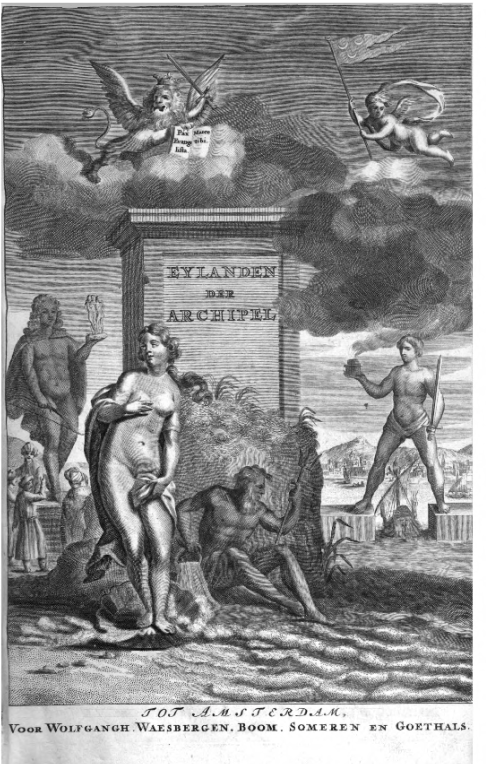
\includegraphics[width=\textwidth]{resources/good_quality}
    \end{subfigure}
    \begin{subfigure}[b]{0.4\textwidth}
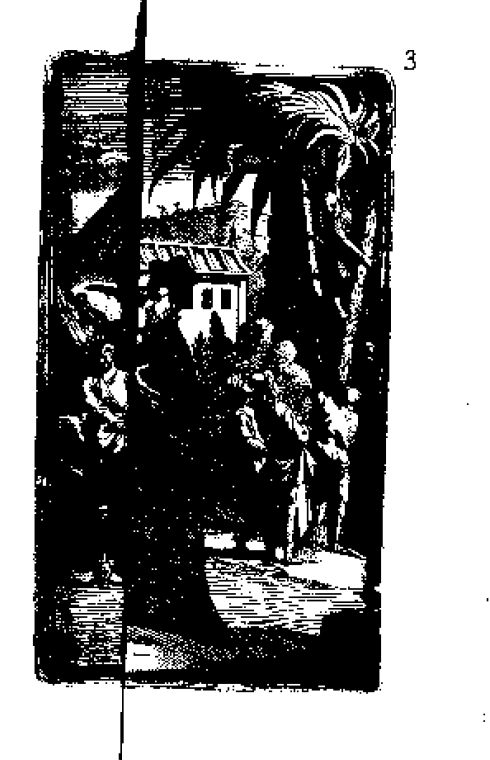
\includegraphics[width=\textwidth]{resources/bad_quality}
    \end{subfigure}
    \caption{The quality differs per book}
    \label{fig:qualityExamples}
\end{figure}


\begin{figure}
\centering
    \begin{subfigure}[b]{0.4\textwidth}

\includegraphics[width=\textwidth]{resources/500_0002}
    \end{subfigure}
    \begin{subfigure}[b]{0.4\textwidth}

\includegraphics[width=\textwidth]{resources/500_0004}
    \end{subfigure}
    \caption{Some pages contain neither text nor image}
    \label{fig:baggerExamples}
\end{figure}


\begin{table}
\centering
\begin{tabular}{l l}
Total amount of pages: & 5960 \\
Mean pages per book: & 236 \\
Standard deviation: & 223 \\
\hline
Total amount of images: & 525 \\
Mean images per book: & 22.8 \\
Standard deviation: & 49.8
\end{tabular}
\caption{Dataset statistics}
\label{tab:statistics}
\end{table}

